\chapter{Feature selection}\label{ch:fs}

We introduce in this chapter the concepts of feature selection and false discovery rate control,
as well as a short review of a few methods that are usually employed.
Finally, we detail the knockoff framework developed by Barber-Candès,
a recent approach to control the false discovery rate when performing feature selection.

\section{Background on feature selection}\label{sec:bfs}

\subsection{Definitions}\label{subsec:fs_defs}

Feature selection is an active area of research in statistics and machine learning.
It primarily consists in identifying the most relevant features (or covariates) explaining an observed variable.
It is closely related to Occam's razor.
More formally, let $\cX$ be a $p$-dimensional random vector representing observed features
and $\cY$ a random target that may depend on $\cX$.
For example, $\cX$ could be the level of expression of the genes of an individual,
and $\cY \in \zoset$ a binary response indicating whether or not the person has some disease.
We wish to find the subset of covariates $\cS \subseteq \fset$ that best explains the target $\cY$,
be it a regression or a classification problem.
To do so, suppose that the joint vector $\left( \cX,\, \cY \right)$ follows some distribution,
that is $\left( \cX,\, \cY \right) \sim \mathcal{P}_{\cX,\, \cY}$.
Even though finding the conditional distribution $\cP_{\cY \mid \cX}$ is beyond hope,
one may be interested in finding on which subset $\cS$ of features $\cP_{\cY \mid \cX}$ depends.
Such a subset is not necessarily unique
\begin{wrapfigure}{l}{0.5\textwidth}
    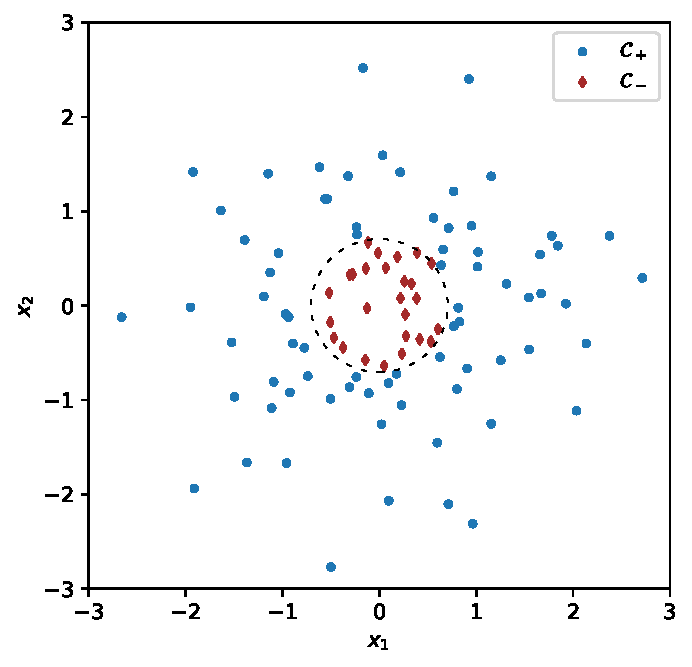
\includegraphics[width=1\linewidth]{figures/fs_subset_not_unique.pdf}
    \caption{
    Illustration of the non-uniqueness of the Markov blanket.
    Here $\cX_1 \sim \cN\left( 0, 1 \right)$,
    $\cX_2 = \cX_1^2$,
    and $\cY$ is $\cC_+$ if $\abs{\cX_1} \geq \frac{1}{2}$,
    $\cC_-$ otherwise.
    Both $\cX_1$ and $\cX_2$ alone are enough to predict $\cY$.
    }
    \label{fig:fs_subset_not_unique}
\end{wrapfigure}
Markov blanket~\cite{markov_blanket}, b~\cite{markov_blanket_fs}.
We define the set of null features $\cH_0 \subseteq \fset$ as follows:
$j \in \cH_0$ if and only if $\cY \independent \cX_j \mid \cX_{-j}$
(where $\cX_{-j}$ denotes that all column entries are kept except the $j$th).
The goal is thus to find a procedure selection a subset of features
$\hat{\cS} \subseteq \fset$.

In practice, one would observe several independent realizations of
$\left( \cX,\, \cY \right)$ and would aggregate them into a feature matrix
$X \in \R^{n \times p}$ of $n$ samples and $p$ features, and a target vector $\yy \in \R^n$ respectively.
The independence of the observations is a credible assumption in many real life settings

\subsection{Motivation}\label{subsec:fs_motivation}

Feature selection may be used in a multitude of contexts and we point out here the main reasons why
one would want to perform it on a dataset.
\begin{enumerate}
    \item Making the model more interpretable.
    It gives insights on the most relevant features to explain the observed target.
    \item Facilitating data visualization.
    As only a small subset of the features is selected,
    projecting it to a low (2 or 3) dimensional space is easier.
    \item Reducing the training time.
    Many machine learning algorithm have a super-linear time complexity in the number of features.
    Pre-selecting a small subsets of those with a cheaper method can noticeably as less\cite{high_dimensional_fs}
    \item Improving the generalization of machine learning models.
    Irrelevant features may only be noise and fitting a model against them at train time
    is prone to over-fitting noise.
    \item Avoiding the curse of dimensionality~\cite{curse_dimensionality}.
    For example, the $k$-nearest neighbors algorithms~\cite{knn} is known to perform badly as the feature space
    dimension increases.
    The number of samples actually has to grow exponentially in the number of features in order for the algorithm
    to perform decently.
\end{enumerate}
Recently, the cost of measuring more features has drastically decreased.
Many datasets, and especially in biology, end up with several dozens of thousands of features.
Most of these features are expected to be insignificant, but there is a priori no reason to eliminate them.
Adding them to the feature matrix is cheap, and it is then the role of the machine learning algorithm
to detect the relevant ones.

\subsection{Techniques}\label{subsec:fst}

A lot of different paradigms and techniques to perform feature selection exist~\cite{intro_fs}
a~\cite{fs_text_classification}.
b\cite{gene_selection_cancer_svm}
c\cite{fs_for_classification}
d\cite{fs_for_classification_a_review}

\subsubsection{Lasso}\label{subsubsec:lasso}

First rediscovered by Tibshirani~\cite{lasso} in 1996,
the Lasso has become increasingly popular because of its capacity to both shrink
the coefficients towards 0 and to select a subset of the features.
It is basically a linear least squares regression whose weights are penalized by their $\ell_1$ norm,
multiplied by some factor $\lambda > 0$.
%
\begin{equation}\label{eq:lasso}
    \hat{\bbeta}(\lambda) =
    \underset{\bb}{\argmin}\;
    \frac{1}{2}\norm{\yy - X\bb}_2^2 + \lambda\norm{\bb}_1
\end{equation}
%
The $\ell_1$ penalty tends to make the weights $\hat{\bbeta}(\lambda)$ sparse as $\lambda$ increases.
Actually, for any feature $j$,
there is a $\lambda_{\min}$ such that for all $\lambda \geq \lambda_{\min}$,
$\hat{\bbeta}_j(\lambda) = 0$.
That wouldn't be the case with an $\ell_2$ penalty,
for which the coefficients tend to $0$ without reaching that value.
This property makes the Lasso particularly suited for feature selection;
just keep the features whose weight is non-zero.
However, the choice of $\lambda$ seems to be arbitrary,
especially as it's not possible to know beforehand how many features will be selected.
The behavior of the path $\lambda \mapsto \hat{\bbeta}(\lambda)$ has been extensively studied,
and the algorithm LARS~\cite{lars} was developed to efficiently compute it
(which is possible because it is piecewise linear).
It allows to compute $\hat{\bbeta}$ for all relevant value of $\lambda$ at a marginal cost.
In practice, the $\lambda$ giving the highest score on a \emph{train} dataset is picked.
The $\ell_1$ regularization can easily be extended to many other estimators than the least squares,
as for example logistic regression or SVMs.

\subsubsection{Sparse center classifiers}

Nearest centroid classification~\cite{centroid_classification} is a very simple classification scheme.
It consists in computing the averages $\btheta^\pm = \sum_{j \in \cI^\pm} \xx_i \in \R^p$
of the data points from the positive and negative classes $\cC^\pm$,
where $\cI^\pm$ contain the positive and the negative points.
A new data point $\xx \in \R^p$ is classified positive or negative depending on its closest average
$\btheta^+$ or $\btheta^-$.
Finding the class averages can be formulated as the following optimization problem.
\begin{equation}\label{eq:centroids_averages}
    \argmin_{\btheta^+, \btheta^-}
        \frac{1}{n^+} \sum_{i \in \cI^+} \big\lVert \xx_i - \btheta^+ \big\rVert^2_2
        + \frac{1}{n^-} \sum_{i \in \cI^-} \big\lVert \xx_i - \btheta^- \big\rVert^2_2
\end{equation}
Note $\Delta$ the decision boundary,
such that $\xx$ is classified $\cC^+$ if $\Delta\left( \xx \right) > 0$ and $\cC^-$ otherwise.
\begin{equation}\label{eq:centroids_boundary}
    \Delta(\xx) = \norm{\xx - \btheta^-}^2_2 - \norm{\xx - \btheta^+}^2_2
\end{equation}
The expression~\ref{eq:centroids_boundary} can be expanded into
$\Delta(\xx) = \norm{\btheta^+}^2_2 + \norm{\btheta^-}^2_2 + 2\xx^\top(\btheta^+ - \btheta^-)$,
making it clear that the decision depends on the feature $j$ if and only if $\btheta^+_j \neq \btheta^-_j$.
Using this observation,\cite{sparse_center_classifiers} introduced a $\ell_0$ penalized version
of~\ref{eq:centroids_averages} that can be solved very efficiently in closed-form.
The authors obtain accuracy scores on par with the ones of the Lasso on the datasets they experiment.
This a sparse centroid classification allows in particular to perform feature selection
by keeping the features $j$ such that $\btheta^+_j \neq \btheta^-_j$.
%
\bigbreak
None of the selection scheme presented above offer strong guarantees regarding
the number of false positives that are detected.
The selected subset $\hat{\cS}$ could potentially be disjoint to $\cS$
if the selection criterion is not adapted to the problem.

\section{False discovery rate control}\label{sec:fdrc}

When performing feature selection one is usually interested in two quantities,
namely the \emph{false discovery rate} (FDR) and the \emph{power}.
Intuitively, the former (resp.\ the latter) assesses the expected proportion of false discoveries
(resp.\ true discoveries) of a selection procedure.

\subsection{Definitions}\label{subsec:fdr_def}

Suppose the conditional probability distribution $\cY \mid \cX$ depends only on a subset of features
$\cS \subset \left\{ 1, \dots, p \right\}$.
A feature selection algorithm outputs a subset $\hat{\cS} \subset \fset$ (which is potentially random)
that it judges to be relevant.
The false discovery proportion (FDR), the false discovery rate (FDR), and the power are defined as follows
\begin{equation}\label{eq:fdr_def}
    \fdp = \frac
        {\big\lvert \big\{ \hat{\cS} \setminus \cS \big\} \big\rvert}
        {\lvert \hat{\cS} \rvert}
    \text{,}\qquad\quad
    \fdr = \Eb{\fdp}
    \text{,}\qquad\quad
    \power = \E{
        \frac
            {\big\lvert \big\{ \hat{\cS} \cap \cS \big\} \big\rvert}
            {\lvert\hat{\cS}\rvert}
    }
\end{equation}
The $\fdp$ merely measures the proportion of features in $\hat{\cS}$ that are not in $\cS$.
It depends on the samples $X$ and $\yy$,
and possibly on the inherent randomness of the selection algorithm.
That is why the $\fdr$ assesses the expectation of this value.
Finally, the $\power$ is the fraction of the important features that were actually discovered, in average.

Even though it is beyond hope to retrieve the whole set $\mathcal{S}$ with no error,
a multitude of techniques attempt to find as many relevant features as possible
(that is, maximizing the power)
while maintaining the FDR under a certain threshold.
The concept of $\fdr$ was first introduced by~\cite{bh} in 1995 and has become increasingly decisive in some
sciences such has biology where the acquisition of a huge number of covariates is frequent.
It is now possible to measure the expression of several dozens of thousands of genes for a given individual.

\subsection{Benjamini–Hochberg-Yekutieli procedures}\label{subsec:bhq}

The Benjamini–Hochberg~\cite{bh} and Benjamini–Yekutieli~\cite{by} schemes are two methods controlling the FDR
that are widely used in practice.
They are closely related to each other but offer different guarantees regarding the effective control of the FDR\@.
BH is less conservative than BY but makes stronger assumptions on the $p$-values it manipulates.

For each feature $j \in \fset$, let $\cH_j$ be the null hypothesis ($j$ does not belong to $cS$),
and $\pvalue_j$ the corresponding $p$-value.
Let $\fdrtarget \in [0, 1]$ be some FDR target that should not be exceeded.
We note $(\pvalue_{(j)})_j$ the sequence of $p$-values in increasing order;
$\pvalue_{(1)} \leq \dots \leq \pvalue_{(p)}$.
Let $m_0$ be the number of true null hypotheses.

\subsubsection{Benjamini–Hochberg}\label{subsubsec:bh}

The Benjamini–Hochberg (BH) procedure was the first method proposed to control the FDR\@.
It consists in the following steps:
\begin{enumerate}
    \item Sorting the $p$-values such that $\pvalue_{(1)} \leq \ldots \leq \pvalue_{(p)}$
    \item Finding the largest $k \in \N$ such that $\pvalue_{(k)} \leq \frac{k \cdot \fdrtarget}{p}$
    \item Rejecting all the hypotheses $\cH_{(j)}$ such that $j \in \left\{ 1, \dots, k \right\}$
\end{enumerate}
In the end, all the features $j$ such that $p_j \leq p_{(k)}$ are selected.
It guarantees that $\fdr \leq \frac{m_0}{p}\fdrtarget$ under the assumption that the $p$-values were computed
independently, which can be very restrictive in many situations.

\subsubsection{Benjamini–Yekutieli}\label{subsubsec:by}

Similarly, the Benjamini–Yekutieli procedure controls the FDR
and does not need the $p$-values independence assumption,
at the cost of a more conservative selection.
It follows the same scheme, namely:
ordering the $p$-values,
finding the largest $k \in \N$ such that $\pvalue_{(k)} \leq \frac{k}{p \cdot c(p)}\fdrtarget$,
and rejecting $\cH_{(j)}$ if $j \leq k$.
Note the additional factor $c(p) \geq 1$, defined in~\ref{eq:by_factor}.
\begin{equation}\label{eq:by_factor}
c(p) = \sum_{j = 1}^p \frac{1}{j}
,\qquad
\fdr \leq \frac{m_0}{p}\fdrtarget
\end{equation}

\begin{figure}[h]
    \centering
    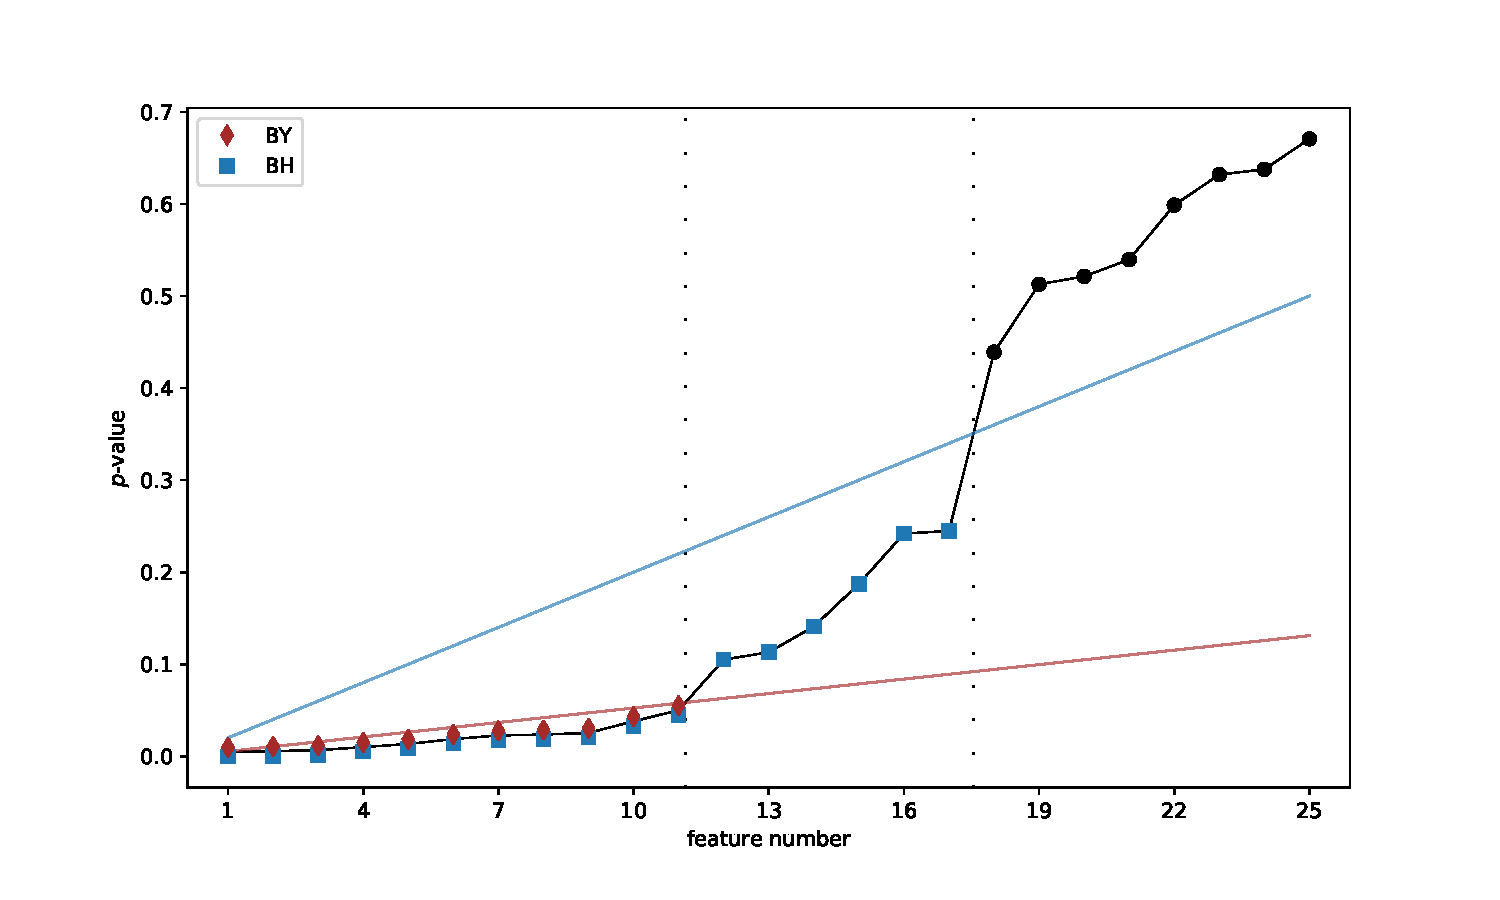
\includegraphics[width=1.\textwidth]{figures/bhy.pdf}
    \caption{
    Illustration of the BH and the BY procedures.
    They are geometrically equivalent to drawing a line of slope $\beta$ going through the origin,
    identifying the last $p$-value under the line, and keeping the features on the left of the intersection point.
    For BH, $\beta = \frac{\fdrtarget}{p}$ (in blue),
    while for BY, $\beta = \frac{\fdrtarget}{p \cdot c(p)}$ (in cyan).
    In this toy example, $\fdrtarget = 0.5$, and it shows that BY is way more conservative than BH.
    }
    \label{fig:bhy}
\end{figure}
\bigbreak
Both procedures are illustrated in figure~\ref{fig:bhy}.
They require $p$-values to be computed, which is not always feasible, especially when $p > n$.
Furthermore, BH and BY have stronger guarantees than desired;
for a desired FDR level $\fdrtarget$,
they ensure that $\fdr \leq \frac{m_0}{p}\fdrtarget$,
and the factor $\frac{m_0}{p}$ might be much smaller than 1.

% \cite{statistical_inference_genome}\cite{resampled_fdr_control}\cite{unified_fdr_control}

\FloatBarrier
\section{FDR control with knockoffs}\label{sec:knockoffs}

In 2015 Barber-Candès introduce the knockoffs framework and extend it later in 2018 to more general settings
(allowing in particular to perform feature selection in the high dimension context).
The goal is to control the false discovery rate as defined in~\ref{eq:fdr_def}, while maintaining a reasonable power.
More formally, let $X \in \R^{n \times p}$ be a a feature matrix and $\yy \in \R^n$ the associated target vector.
Suppose $\yy$ depends only on the subset of features $\cS \subseteq \fset$.
Given some $\fdr$ target $\fdrtarget \in [0, 1]$, we wish to find a procedure such as, in average,
the false discovery proportion is smaller that $\fdrtarget$, i.e. $\fdr \leq q$.
To do so, the key idea is to construct for each original feature $X_j$, $j \in \fset$,
a knockoff (that is to say, fake) feature $\tilde{X}_j$ which is known to be out of the model.
Original features are then selected only if they prove to be more significant than their knockoff counterparts.

Note $\Sigma = X^\top X$.

To compare a feature and its knockoff several quantities will be computed by interchanging them.
For this reason, we define in~\ref{def:swap} the $\swap$ operator.
\begin{definition}\label{def:swap}
    \text{($\swap$ operator)}
    Given two matrices $A,\,B \in \R^{n \times p}$ of same size,
    we define the $\swap$ operator on the concatenated matrix $\big[ A, B \big]$ as follows.
    For a any subset of indices $S \subseteq \left\{ 1, \dots, p \right\}$,
    $\big[ A, B \big]_{\swap(S)}$ is the transformed matrix where the columns $A_j$ and $B_j$ were swapped for all
    $j \in S$.
\end{definition}

In the following sections, we are going to detail principal aspects of the construction of the knockoff features,
the computation of statistics for both original and knockoff features,
and the feature selection itself, based on those statistics.

\subsection{Knockoffs construction}\label{subsec:kc}

In 2015, Barber-Candès introduced first the \textit{fixed}-X knockoffs variable selection procedure.
It relies on the creation of fake features satisfying some correlation constraints with the original features.
Unfortunately, it can only perform adequately when $n \geq 2p$,
even though it can be partially extended to the cases where $n \geq p$.
In 2018, Candès proposed an extension of the framework called \textit{model}-X knockoffs,
in which fake features are sampled from a learned distribution.
Despite the restriction of \textit{fixed}-X knockoffs, that method is still appealing as the construction of the
knockoff variables is straightforward (but costly).
On the other hand, \textit{model}-X knockoffs work in higher feature dimensions
but need an estimation of the distribution that generated the data,
which is a hard problem in general.
We will focus on the construction of \textit{model}-X knockoffs as we are principally interested in the
high dimensional setting.

In this section, let $(\cX, \cY)$ be a pair of random variables,
$\cX$ being composed of $p$ features,
and $\cY$ the associated target in $\R$.
We suppose that the feature matrix and the target vector $(X,\, \yy)$ are composed of samples from $(\cX,\, \cY)$.
We wish to build knockoff features $\tX \in \R^{n \times p}$, and to do so we are going to sample from a
random variable $\tcX$ built such that $\big[ \cX; \tcX \big]$
follows the properties~\ref{itm:cond_swap} and~\ref{itm:cond_indep} defined thereafter.

\subsubsection{General case}

\begin{definition}
    \text{(model-$X$ knockoffs)}
    Given random vector $\cX \in \R^p$ of features,
    a random vector $\tcX \in \R^p$ is said to be model-$\cX$ knockoffs with respect to $\cY$
    if it satisfies the two following properties:
    \begin{enumerate}[label=\textbf{S.\arabic*},ref=S.\arabic*]
        \item \label{itm:cond_swap} For any $S \subseteq \fset$,
            $\big[ \cX; \tcX \big]^\top_{\swap(S)} \distreq \big[ \cX; \tcX \big]^\top$
        \item \label{itm:cond_indep} $\tcX \independent \cY \mid \cX$
    \end{enumerate}
\end{definition}
Intuitively, the condition~\ref{itm:cond_swap} ensures that a knockoff feature is sufficiently
close to its associated original feature so that swapping them doesn't change the distribution of the
concatenated random vector.
The independence condition~\ref{itm:cond_indep} states that the knockoff features
carry no additional information on $\cY$, given $\cX$.
It is trivially satisfied if $\tX$ is built without exploiting $\yy$.
However, constructing knockoffs meeting the first distribution equality is practically infeasible in general.
\begin{remark}
    Constructing the knockoffs feature matrix $\tX \in \R^{n \times p}$.
    It must satisfy two conditions, namely:
    \begin{align*}
        &{\tX}^\top\tX = \Sigma,
        \\
        &X^\top\tX = \Sigma - \diag\{\bs\}
        \text{ where } \bs \text{ is a non negative vector.}
    \end{align*}
    It ensures that $\tX$ has the same covariance as the original matrix $X$
    and that the correlation between distinct original and knockoff variables is
    the same as the correlation between the two originals.
\end{remark}

\subsubsection{Gaussian case}

In the particular case where $\cX$ is multivariate gaussian, the exact distribution of $\tcX$ can be derived.
\begin{proposition}
    Suppose that $\cX \sim \cN(\bmu, \Sigma)$.
    If $\tcX$ is a random variable such that
    \begin{equation*}
        \big[ \cX; \tcX \big] \sim \cN\bigg(\begin{bmatrix} \bmu\\ \bmu \end{bmatrix}, \Omega\bigg)
        ,\quad\text{where }\quad
        \Omega = \begin{bmatrix}
             \Sigma & \Sigma - \diag \bs\\
             \Sigma - \diag \bs & \Sigma
        \end{bmatrix}
        \quad\text{for some }
        \bs \in \R^p,
    \end{equation*}
    then $\big[\cX, \tcX \big]$ satisfies the $\swap$ property~\ref{itm:cond_swap},
    provided that $\Omega$ is positive semidefinite (so that it is indeed a covariance matrix).
\end{proposition}\label{prop:gaussian_knockoffs}
In the proposition~\ref{prop:gaussian_knockoffs},
$\bs \in \R^p$ can be any vector such that $\Omega \succeq \0$.
We will come back later to the choice of $\bs$ which is actually crucial.
For now, assume that $\bs$ satisfies this assumption.
This result gives a way of constructing the knockoff features from $X$.
Indeed, as $\big[ \cX; \tcX \big]$ is multivariate normal, we may compute the exact distribution of
$\tcX \mid \cX$ with classical formulas~\cite{conditional_normal} as shown in~\ref{eq:conditional_gaussian_knockoffs}.
\begin{equation}\label{eq:conditional_gaussian_knockoffs}
    \tcX \mid \cX \sim \cN\left( \bupsilon, \Upsilon \right)
    ,\qquad\text{where}\quad
    \begin{cases*}
        \bupsilon = \cX - \cX\Sigma^{-1}\diag(\bs)\\
        \Upsilon = \diag(\bs)\left( 2\mI_{p \times p} - \Sigma^{-1}\diag(\bs) \right)
    \end{cases*}
\end{equation}
To put this into practice, one would compute the empirical mean
$\hat{\bmu} \in \R^p$ and covariance $\hat{\Sigma} \in \R^{p \times p}$ of $\cX$
using the observed feature matrix $X$.
Then, each row of $\tX$ is sampled according to a gaussian distribution $\cN\left( \bupsilon, \Upsilon \right)$
whose parameters are described in~\ref{eq:conditional_gaussian_knockoffs}.
Note in particular that the construction process is random;
if it is repeated, it may very well return different knockoffs, and thus different
selected features.
Because of this instability, several attempts~\cite{improve_stability_knockoffs} to fix it by
aggregating several knockoff samples.

Depending on the prior on the data and on the available computing power,
several algorithms may be used to estimate the covariance matrix $\Sigma$.
The empirical estimator is cheap but known to be unstable when $p > n$.
Shrunk estimations like Ledoit-Wolf~\cite{ledoit_wolf} provide good results.
\bigbreak
The gaussian hypothesis is obviously rarely verified in practice but yields acceptable results even when
$\cX$ is far from gaussian.
It partly comes from the fact that, rather than constructing $\tcX$ to respect~\ref{itm:cond_swap},
a weaker condition would be to enforce $\big[ \cX, \tcX \big]$ and $\big[ \cX, \tcX \big]_{\swap(S)}$ to have the
same first two moments (mean and covariance).
It turns out to be the case if $\tcX \mid \cX$ is constructed as described in~\ref{eq:conditional_gaussian_knockoffs}.
In the remaining of this master thesis, we will restrain ourselves to the gaussian hypothesis.

The first knockoff paper~\cite{fixed_x_knockoffs} introducing the \textit{fixed}-X knockoffs relied on similar correlation
properties between the original and the knockoff features.
It however imposed $p \leq n$ and fewer statistics would yield theoretical guarantees regarding the FDR control
of the procedure.
In the reminding, we will only consider \textit{model}-X knockoffs as we are interested in the high dimensional
setting.
Moreover, \textit{model}-X knockoffs tend to give higher power experimentally compared to their \textit{fixed}
counterparts.

Note that generating knockoffs requires an estimation of the distribution of $\cX$ only,
and not $\cY \mid \cX$ as most methods would.
It is particularly appealing because labeling data is often the most costly part,
while acquiring samples $\xx \sim \cX$ is easier.
Unlabeled samples are thus valuable.

\subsection{Statistics computation}\label{subsec:ksc}

\subsubsection{General principle}\label{subsubsec:scg}

Given the original feature matrix and the sampled knockoffs $X,\, \tX \in \R^{n \times p}$,
statistics $w_j$ for all $j \in \fset$ are computed.
These statistics must satisfy the \emph{flip-sign} technical condition~\ref{def:flip_sign} for the method to work,
but a wide variety of choices is possible as will be shown.
\begin{definition}\label{def:flip_sign}
\text{(flip-sign property)}
A statistics function $\omega \colon \R^{n \times 2p} \times \R^n \to \R^p$
is said to follow the flip-sign property if for any $S \subseteq \fset$ and any $j \in \fset$,
\begin{equation*}
    \omega_j\big( \big[ X, \tX \big]_{\swap(S)},\, \yy \big) = \begin{cases*}
        -\omega_j\big( \big[ X, \tX \big]_{\swap(S)},\, \yy \big) &\quad\text{if $j \in S$.}\\
        \omega_j\big( \big[ X, \tX \big]_{\swap(S)},\, \yy \big) &\quad\text{otherwise.}
    \end{cases*}
\end{equation*}
\end{definition}

\subsubsection{Statistics aggregation}\label{subsubsec:ksa}

Constructing statistics satisfying the \emph{flip-sign} property~\ref{def:flip_sign} is actually straightforward
as a simple scheme leads to such statistics.
The idea is to build statistics for each original and each knockoff feature, and then aggregate them.
First construct statistics $[ \zz ; \tilde{\zz} ] = \zeta\big( \big[ X, \tX \big],\, \yy \big)$
with some function $\zeta \colon \R^{n \times 2p} \times \R^n \to \R^{2p}$ satisfying
\begin{equation}\label{eq:swap_cond}
    [ \zz ; \tilde{\zz} ]_{\swap(S)} = \zeta\big( \big[ X, \tX \big]_{\swap(S)},\, \yy \big)
    ,\quad
    \forall S \subseteq \fset
\end{equation}
The statistics $z_j$ (resp. $\tilde{z}_j$) indicates how significant the original (resp.\ knockoff) feature $j$ is.

Then aggregate for each $j \in \fset$ the statistics of the original feature $z_j$ and the one of the corresponding
knockoff $\tilde{z}_j$ with an antisymmetric function $a_j \colon \R\times\R \to \R$,
that is, set $w_j = a_j(z_j, \tilde{z}_j)$.
Basically any antisymmetric function could work, but some choices lead to better statistics.
As for the function $\zeta$, it only needs to satisfy the \emph{swap} property~\ref{eq:swap_cond}.
This condition may seem restrictive but a large number of choices are actually valid.

Computing antisymmetric statistics $\ww \in \R^p$ where $\forall j = 1, \dots, p$, $w_j$
indicates how more important an original feature $j$ is compared to its associated knockoff.
Several mappings are possible, for example:
\begin{itemize}
    \item $w_j = z_j - \tilde{z}_j$ (experimentally gives highest power)
    \item $w_j = \max(z_j, \tilde{z}_j) \times \sign(z_j - \tilde{z}_j)$ (first proposed in 2015)
    \item $w_j = \log\frac{z_j}{\tilde{z}_j}$
\end{itemize}

\subsubsection{Examples}\label{subsubsec:sce}

A few examples of statistics relying on the aggregation trick are presented in this subsection.
In~\cite{fixed_x_knockoffs}, Barber-Candès suggest after empirical observations the use of the
Lasso Signed Max (LSM) statistics defined as follows.
Let $\hat{\bbeta}(\lambda)$ be the coefficients of a Lasso model with penalty coefficient $\lambda > 0$.
As mentioned in subsection~\ref{subsubsec:lasso},
all the coefficients are null starting from $\lambda = \inf$,
and will potentially change as $\lambda \to 0$.
Then define $z_j$ to be the highest value of $\lambda$ such that .
Intuitively, it is the first $\lambda$ such that the feature enters in the model.
\begin{equation}
    z_j = \sup\{\lambda \mid \hat{\bbeta}_j(\lambda) \neq 0\}
    ,\qquad\qquad
    \hat{\bbeta}(\lambda) =
        \underset{\bb}{\argmin}\;
        \frac{1}{2}\norm{\yy - X\bb}_2^2 + \lambda\norm{\bb}_1
\end{equation}
There are other ways to compute the $z_j$ statistics.
It would for example be possible to train a regressor and take the absolute values of its coefficients.

\subsection{Features selection}\label{subsec:kfs}

The selection itself requires the computation of a data-dependent threshold $\tau$
conditioned by the target FDR $\fdrtarget$, as defined in~\ref{eq:knock_thres} and~\ref{eq:knockp_thres}.
Finally, features $j$ whose statistics $w_j$ are above the threshold are selected;
$\hat{\cS} = \left\{ j \mid w_j \geq \tau \right\}$.
Depending on how selective we want the procedure to be, the threshold $\tau$ can be adapted,
and leads to different guarantees regarding the control of the FDR\@.
Let's first define a modified version of the FDR\@.
\begin{definition}\label{def:mfdr}
Given an estimate $\hat{\cS}$ of $\cS$ and a desired target false discovery rate $q \in [0, 1]$,
we define the modified $\fdr$ as follows:
\begin{equation*}
    \mfdr = \E{
    \frac
    {\abs{\left\{ j \mid j \in \hat{\cS} \setminus \cS \right\}}}
    {\lvert\hat{\cS}\rvert + 1 / q}
    }
\end{equation*}
\end{definition}
As $q \leq 1$, $\mfdr$ as defined in~\ref{def:mfdr} is always smaller than the actual $\fdr$.
But if the target threshold $q$ is not too low, and if many features are selected by the procedure,
the modified version of the FDR is close enough to the true value.
Controlling it is then relevant.
\begin{definition}
    (knockoff and knockoff+ thresholds)
    \begin{align}
        \tau &=
        \min\left\{
        t > 0 \mid \frac{\abs{j \mid w_j \leq -t}}{\abs{j \mid w_j \geq t}} \leq q
        \right\}\label{eq:knock_thres}\\
        \tau^+ &=
        \min\left\{
        t > 0 \mid \frac{1 + \abs{j \mid w_j \leq -t}}{\abs{j \mid w_j \geq t}} \leq q
        \right\}\label{eq:knockp_thres}
    \end{align}
\end{definition}

\begin{theorem}
    Construct $\hat{\cS} = \left\{ j \mid w_j \geq \tau \right\}$
    and $\hat{\cS}^+ = \left\{ j \mid w_j \geq \tau^+ \right\}$.
    Then,
    \begin{equation}
        \mfdr\left[ \hat{\cS} \right] \leq q
        ,\qquad
        \fdr\left[ \hat{\cS}^+ \right] \leq q
    \end{equation}
\end{theorem}
%
\subsection{Bottlenecks}\label{subsec:kb}

Despite the nice theoretical guarantees on the $\fdr$ control that the knockoff procedure proposes,
two bottlenecks hurt its performances in the high dimensional setting.

\subsubsection{SDP}\label{subsubsec:bot_sdp}

Knockoff features are sampled according to the distribution~\ref{eq:conditional_gaussian_knockoffs},
and the results hold for any $\bs \in \R^p$ such that the covariance matrix is semidefinite positive.

\begin{proposition}
    Let $\Omega = \begin{bmatrix}
                      \Sigma & \Sigma - \diag \bs\\
                      \Sigma - \diag \bs & \Sigma
    \end{bmatrix}$.
    Then $\Omega \succeq \0_{p \times p}$ if and only if $2\Sigma \succeq \diag \bs \succeq \0$.
\end{proposition}

\begin{proof}
    Note $D = \diag\bs$.
    By computing the Schur complement~\cite{schur_complement}
    $\Omega_{/\Sigma} = 2D - D\Sigma^{-1}D$,
    $\Omega \succeq \0$ is equivalent to $\Omega_{/\Sigma} \succeq \0$.
    Define $M$ and its Schur complements as follows
    \begin{equation*}
        M = \begin{bmatrix}
            2D & D\\
            D & \Sigma
        \end{bmatrix}
        ,\qquad\qquad
        \begin{cases*}
            M_{/2D} = \Sigma - \frac{1}{2}D\\
            M_{/\Sigma} = 2D - D\Sigma^{-1}D
        \end{cases*}
    \end{equation*}
    Finally, $\Omega_{/\Sigma} = M_{/\Sigma}$ is p.s.d.\ if and only if both $\Sigma - \frac{1}{2}D$ and $D$ are p.s.d.
\end{proof}

\subsubsection{Statistics computation}\label{subsubsec:bot_stats}

and could take advantage of sparse naive Bayes to run faster.
\bigbreak
These two bottlenecks make the .
The following chapters tackle these two issues by proposing fast statistics computation.
From now, only binary classification problems will be considered, where the label $y$ takes values
in $\left\{ \cC^+,\, \cC^- \right\}$.

\subsection{Python implementation}\label{subsec:python_implementation}

Barber-Candès (along with other coauthor) provided a R implementation
of the knockoff framework\footnote{
The package page can be found at this address \url{https://cran.r-project.org/web/packages/knockoff/index.html}.
}.
To the best of our knowledge, no unified Python implementation
Scikit-Learn~\cite{sklearn}
